\message{ !name(../thesis_main.tex)}%%% thesis_main.tex --- 

%% Author: garamonfok@gros
%% Version: $Id: thesis_main.tex,v 0.0 2011/10/09 18:39:32 garamonfok Exp$
%%% master.tex --- 

%% Author: garamonfok@gros
%% Version: $Id: style.sty,v 0.0 2011/10/09 18:39:32 garamonfok Exp$


%%%%%%%%% Document class declaration  %%%%%%%%%%%%%%%%%%%%%%%%%%%%%%%%%%%%%%%%%%

% really strange... but the only way to load xcolor together with tikz package
% usually loaded as usepackage[table]{xcolor}
% thisis for defining rowcolors
\PassOptionsToPackage{table}{xcolor}
\documentclass[english,b5paper,11pt]{scrbook}

  
%%%%%%%%% Load my style  %%%%%%%%%%%%%%%%%%%%%%%%%%%%%%%%%%%%%%%%%%%%%%%%%%%%%%%
\usepackage{../style/thesis}

%%%%%%%%%%%%%%%%%%%%%%%%%%%%%%%%%%%%%%%%%%%%%%%%%%%%%%%%%%%%%%%%%%%%%%%%%%%%%%%%
%%%%%%%%% Thesis starts here  %%%%%%%%%%%%%%%%%%%%%%%%%%%%%%%%%%%%%%%%%%%%%%%%%%
%%%%%%%%%%%%%%%%%%%%%%%%%%%%%%%%%%%%%%%%%%%%%%%%%%%%%%%%%%%%%%%%%%%%%%%%%%%%%%%%
 
\begin{document}

\message{ !name(Material_Methods/material_methods.tex) !offset(-29) }
%%% material_methods.tex --- 

%% Author: garamonfok@gros
%% Version: $Id: material_methods.tex,v 0.0 2011/10/09 18:39:32 garamonfok Exp$

\section{Measuring DNA complexity}

\subsection{The complexity ratio and complexity value}
\label{sec:compl-ratio-compl}

Complexity Ratio (CR) is defined by a classical formula used in data compression \cite{Adjeroh2008}. It is the result of three transformation steps of a given sequence. First, the \mygls{Burrows-Wheeler} transform (BWT) \cite{Burrows1994}, second the Move To Front (MTF) \cite{Ryabko1980} algorithm and finally the summarizing of the unexpected dispersion of the values obtained through Shannon's entropy \cite{Shannon1948} (see \autoref{tab:cr_example} for an example of the process). Thus the CR is Shannon's entropy of a transformation or digestion of the sequence. The purpose of this transformation is to reveal the regularities in a sequence. Shannon's entropy is zero --this is the minimum-- only when a sequence consists just of a single repeated symbol, which is the simplest possible combinatorial structure. Conversely, when entropy is equal to one (the maximum entropy), it indicates that the sequence has a random-like combinatorial structure. 

\begin{table}[!ht]
  \scriptsize
  \rowcolors{1}{white}{lightgray}
  Given a sequence, $seq=AACCTTCGTAGCATGG$:
  \begin{center}
      \begin {tabular}{clc}
        \hline
        \textbf{\#} & \textbf{Rotating sequence} & \textbf{\textit{I.}} \\ \hline
        0  & AACCTTCGTAGCATG\textbf{G}$|$ & 0  \\
        1  & ACCTTCGTAGCATGG$|$\textbf{A} & 1  \\
        2  & CCTTCGTAGCATGG$|$A\textbf{A} & 5  \\
        3  & CTTCGTAGCATGG$|$AA\textbf{C} & 7  \\
        4  & TTCGTAGCATGG$|$AAC\textbf{C} & 15 \\
        5  & TCGTAGCATGG$|$AACC\textbf{T} & 13 \\
        6  & CGTAGCATGG$|$AACCT\textbf{T} & 6  \\
        7  & GTAGCATGG$|$AACCTT\textbf{C} & 11 \\
        8  & TAGCATGG$|$AACCTTC\textbf{G} & 12 \\
        9  & AGCATGG$|$AACCTTCG\textbf{T} & 2  \\
        10 & GCATGG$|$AACCTTCGT\textbf{A} & 9  \\
        11 & CATGG$|$AACCTTCGTA\textbf{G} & 4  \\
        12 & ATGG$|$AACCTTCGTAG\textbf{C} & 3  \\
        13 & TGG$|$AACCTTCGTAGC\textbf{A} & 14 \\
        14 & GG$|$AACCTTCGTAGCA\textbf{T} & 10 \\
        15 & G$|$AACCTTCGTAGCAT\textbf{G} & 8  \\ \hline
      \end {tabular}
    {\Large\pointer}
      \rowcolors{1}{white}{lightgray}
      \begin {tabular}{ c }
        \hline
        \textbf{BWT} \\ \hline
        G \\
        A \\
        T \\
        C \\
        G \\
        A \\
        T \\
        C \\
        G \\
        A \\
        T \\
        C \\
        G \\
        T \\
        A \\
        C \\ \hline
      \end {tabular}
    {\Large\pointer}
      \rowcolors{1}{white}{lightgray}
      \begin {tabular}{ c c c c c }
        \hline
        \multicolumn{4}{c}{\textbf{Char. list}} & \textbf{MTF} \\ \hline
        \textbf{G} & a & t & c & 0 \\
        G & \textbf{A} & t & c & 1 \\
        A & g & \textbf{T} & c & 2 \\
        T & a & g & \textbf{C} & 3 \\
        C & t & a & \textbf{G} & 3 \\
        G & c & t & \textbf{A} & 3 \\
        A & g & c & \textbf{T} & 3 \\
        T & a & g & \textbf{C} & 3 \\
        C & t & a & \textbf{G} & 3 \\
        G & c & t & \textbf{A} & 3 \\
        A & g & c & \textbf{T} & 3 \\
        T & a & g & \textbf{C} & 3 \\
        C & t & a & \textbf{G} & 3 \\
        G & c & \textbf{T} & a & 2 \\
        T & g & c & \textbf{A} & 3 \\
        A & t & g & \textbf{C} & 3 \\ \hline
      \end {tabular}
  \end{center}
  \pointer 
  $\:\:CR(seq) = E(MTF(BWT(seq))) = E(0, 1, 2, 3, 3, 3, 3, 3, 3, 3, 3, 3, 3, 2, 3, 3) = 0.593$
  \caption [CR explained by example]{%
    \textbf{CR explained by example.}\\These three tables summarizes the steps needed to obtain the final sequence of number from which we will finally compute Shannon's entropy. 1) The table on the left corresponds to the BWT. Original sequence is rotated sequentially (first character moved to back) resulting in different strings, as many as characters in the sequence. The resulting sequences are then sorted in lexicographic order. The ''\textit{I.}'' column corresponds to the Index of this ordering (e.g.: the third sequence here in original order ''\#'' takes the fifth position in lexicographic order). 2) The table in the center corresponds to the result of the BWT, that is the last character of previous sequences ordered as explain. 3) The table on the right corresponds to the application of the MTF algorithm. Starting from a sequence of all character named here ''Char. list'' (our four nucleotides in this case), the MTF will get the index of the current nucleotide from the BWT (upper case bold letter) in the ''Char. list''. In a second step, for the next iteration, MTF will transform the ''Char. list'' bringing to front the character present in previous BWT result (upper case letter).\\
    Finally, we compute the Shannon's entropy of the values obtained by the MTF that results in our CR (the CV is obtained by multiplying CR by the length of the sequence).}
  \label{tab:cr_example}
\end{table}

Algorithmically, the BWT of a given sequence is a permutation of the symbols that represents the lexicographic order of all possible rotations of the sequence. The MTF transforms a given sequence into a list of numbers, operating from left to right, and maintaining a stack of recently used symbols. Each number is an index in the stack and denotes an alphabet symbol. Shannon's entropy maps a sequence into a real number between zero and one. It weights the frequency of the alphabet symbols in a given sequence. For each symbol $i$ in the alphabet, let $p_{(i)}$ be the probability of finding $i$ in the sequence $s$; $N_i$ the number occurrences of $i$ in $s$ and $length(s)$ the total length of the sequence $s$: 

\begin{equation} \label{eq:prob_seq}
p_{(i)} = \frac {N_i}{length(s)}
\end{equation}

For DNA alphabet entropy is defined as:

\begin{equation} \label{eq:entropy}
E(s) = -\sum_{i=0}^3p_{(i)} \times log_4(p_{(i)})
\end{equation}

With $i$ the index of characters used, for nucleotides from 0 to 3. Thus the CR can be factorize as:

\begin{equation} \label{eq:cr}
CR(s) = E(MTF(BWT(s)))
\end{equation}

The complexity value (CV) of a sequence is its CR times the number of
characters in this sequence (here $s$):

\begin{equation} \label{eq:cv}
CV(s) = E(MTF(BWT(s))) \times length(s)
\end{equation}

As the CV of a sequence depends on the transformation of the MTF applied to the whole sequence, its computation impede the use of parts of the sequence independently.

\subsection{Complexity in strings}
\label{sec:complexity-strings}

\subsubsection{Genomic sequences}
\label{sec:genomic-sequences}

Complete genomes of 54 species were downloaded from \textit{NCBI} database resource \cite{Sayers2009} and \textit{Ensembl} Genome Project \cite{Flicek2011}. Fourteen major groups of taxa were selected: virus, phages, bacteria, archaea, fungi, amplicomplexa, heterokonta, amebozoa, urochordates, invertebrates, plants, fishes, birds, and mammals. Species among taxa were chosen to their interest as model species or the presence of particular biological features such as: variation in genome size, ancestral or recent polyploidy, living in extreme environments, living as intracellular parasites, gene expansion, genome reduction, RNA or single-strand DNA genomes, and synthetic genomes \autoref{tab:genome}. Eukaryote genomes with coverage of 6$\times$ or greater were chosen. Sexual chromosomes were excluded from the analysis, and ambiguous ``N'' characters were removed from sequences, and excluded in the measure of chromosome length. Eukaryote's genome complexity was calculated over concatenated chromosomes.

Complexity in biological sequences was computed in the +1 strand. Analysis of -1 strand provided no differences in results.

Random sequences with different ploidy levels were also needed for the study, they were generated with \textit{python}\cite{VanRossum2003}. Complexity value of biological sequences and random sequences was computed with the DNA alphabet of four letters.

\subsubsection{Annotation of repetitive elements}
\label{sec:annot-repet-elem}

Interspersed repeats and low complexity DNA sequences were screened and mapped in chromosomes of thirty different eukaryotes using RepeatMasker \cite{Smit2010} (see details of RepeatMasker output for individual species in \autoref{cha:repe-summ-outp}). Complexity of major families of repetitive elements such as DNA \myglspl{transposon}, \myglspl{LTR}, \myglspl{LINE}, \myglspl{SINE}, satellites and exons, introns, and complete genes (considering untranslated regions) was computed after concatenation of all elements in chromosomes excluding.  An example of summary file given by RepeatMasker is shown in  \autoref{cha:repe-summ-outp}.

Here is a listing of the hierarchy of main classes and subclasses annotated by the software:
\begin{itemize}
\item Transposable Element
  \begin{itemize}
  \item DNA \mygls{transposon}:
    \begin{inparaenum}[\itshape 1-]
    \item Mariner / Tc1
    \item hAT
    \item MuDR
    \item EnSpm
    \item piggyBac
    \item P
    \item Merlin
    \item Harbinger
    \item Transib
    \item Novosib
    \item Mirage
    \item Helitron
    \item Polinton
    \item Rehavkus
    \item Kolobok
    \item ISL2EU
    \item Chapaev
    \item Crypton
    \item Sola
    \item Zator
    \item Ginger1
    \item Ginger2 / TDD
    \item Academ 
    \end{inparaenum}
  \item \myGls{LTR} \myGls{retrotransposon}:
    \begin{inparaenum}[\itshape 1-]
    \item Gypsy
    \item Copia
    \item BEL
    \item DIRS 
    \end{inparaenum}
  \item Endogenous Retrovirus:
    \begin{inparaenum}[\itshape 1-]
    \item ERV1
    \item ERV2
    \item ERV3
    \item Lentivirus 
    \end{inparaenum}
  \item Non-\myGls{LTR} \myGls{retrotransposon}:
    \begin{inparaenum}[\itshape 1-]
    \item \mygls{SINE} (\mygls{SINE}1 / 7SL, \mygls{SINE}2 / tRNA, \mygls{SINE}3 / 5S and \mygls{SINE}4)
    \item CRE
    \item NeSL
    \item R4
    \item R2
    \item L1
    \item RTE
    \item I
    \item Jockey
    \item CR1
    \item Rex1
    \item RandI
    \item Penelope
    \item Tx1
    \item RTEX
    \item Crack
    \item Nimb
    \item Proto1
    \item Proto2
    \item RTETP
    \item Hero
    \item L2
    \item Tad1
    \item Loa
    \item Ingi
    \item Outcast
    \item R1
    \item Daphne
    \item L2A
    \item L2B
    \item Ambal
    \item Vingi
    \item Kiri 
    \end{inparaenum}
  \end{itemize}
\item Simple Repeat
  \begin{itemize}
  \item Satellite:
    \begin{inparaenum}[\itshape 1-]
    \item SAT
    \item MSAT 
    \end{inparaenum}
  \end{itemize}
\item Pseudogene
  \begin{itemize}
  \item rRNA
  \item tRNA
  \item snRNA 
  \end{itemize}
\item Integrated Virus
  \begin{itemize}
  \item DNA Virus
  \item Caulimoviridae 
  \end{itemize}
\end{itemize}


\subsubsection{Human texts}
\label{sec:human-texts}

Short stories, books and complete works in its original languages were downloaded from Project Gutenberg (\myurl{http://www.gutenberg.org/}). To automatically detect the alphabet size in texts (including mathematical and punctuation symbols) we run \textit{COMPL} program with ``auto'' option, that takes into account all characters found, including mathematical symbols, and different punctuation signs. 

\subsubsection{Complexity in windows}
\label{sec:complexity-windows}

To study complexity along chromosomes, a sliding window method shifting along chromosomes in overlapping units of 1.0 Kb to 100 Mb was performed. Standard linear models and linear models with interactions were run in R language \cite{Team2008}.

\subsection{Simulations}
\label{sec:simulations}

We performed four kinds of experiments where CV and CR were computed. First: random polyploid construction of sequences of various sizes and ploidy levels ($1\times$ to $10\times$). Second: the evolution along 40 million generations by constant neutral mutation rate of $1.0e^{-08}$ mutations per site per generation (this value is in between the mutation rate estimated for {\it Homo sapiens}: $2.5e^{-08}$ \cite{Nachman2000} , and \textit{Arabidopsis thaliana}: $7.1e^{-09}$ \cite{Ossowski2010}) over random sequences, and chromosomes of \textit{Zea mays} and \textit{Sorghum bicolor}. Third: the evolution along 50,000 generations of random polyploid genomes of different sizes (100Kb, 1Mb, 10Mb) by 1.0 Kb transpositions between chromosomes. The number of transposition per generation was set as a constant function of genome size (genome size over 1,000). Last: the concatenation and shuffling (computed with the \textit{python} base function: ``shuffle'') of all repetition instances in chromosomes for main repetitive families, and genes were considered. Complexity value and ratio were computed every 100 generations. 

\section{Measuring dynamics of genetic species}
\label{sec:meas-dynam-genet}

\subsection{Genomes}
\label{sec:genomes}

For the study of dynamics of genomic elements Genomic sequences of 31 species from unicellular eukaryotes to mammals were used, all were extracted from previous work see  \autoref{sec:complexity-strings} and \autoref{tab:genome}. The complete list of species used is: \begin{inparaenum}[\itshape 1)]
\item \textit{Gallus gallus}            (Birds)
\item \textit{Taeniopygia guttata}      (Birds)
\item \textit{Danio rerio}              (Fishes)
\item \textit{Oryzias latipes}          (Fishes)
\item \textit{Tetraodon nigroviridis}   (Fishes)
\item \textit{Saccharomyces cerevisiae} (Fungi)
\item \textit{Anopheles gambiae}        (Invertebrates)
\item \textit{Caenorhabditis elegans}   (Invertebrates)
\item \textit{Drosophila melanogaster}  (Invertebrates)
\item \textit{Tribolium castaneum}      (Invertebrates)
\item \textit{Bos taurus}               (Mammals)
\item \textit{Canis familiaris}         (Mammals)
\item \textit{Equus caballus}           (Mammals)
\item \textit{Homo sapiens}             (Mammals)
\item \textit{Macaca mulatta}           (Mammals)
\item \textit{Monodelphis domestica}    (Mammals)
\item \textit{Mus musculus}             (Mammals)
\item \textit{Pan troglodytes}          (Mammals)
\item \textit{Pongo abelii}             (Mammals)
\item \textit{Rattus norvegicus}        (Mammals)
\item \textit{Arabidopsis lyrata}       (Plants)
\item \textit{Arabidopsis thaliana}     (Plants)
\item \textit{Brachypodium distachyon}  (Plants)
\item \textit{Oryza sativa}             (Plants)
\item \textit{Populus trichocarpa}      (Plants)
\item \textit{Sorghum bicolor}          (Plants)
\item \textit{Zea mays}                 (Plants)
\item \textit{Dictyostelium discoideum} (unicellular Eukaryotes)
\item \textit{Plasmodium falciparum}    (unicellular Eukaryotes)
\item \textit{Thalassiosira pseudonana} (unicellular Eukaryotes)
and \item \textit{Ciona intestinalis}   (Urochordate)
\end{inparaenum}.

\subsection{Mining of Genetic Elements}

For this study, GEs were divided into 2 categories, repetitive elements and functional elements.

\subsubsection{Repetitive Elements}

Repetitive elements were retrieved as \autoref{sec:annot-repet-elem}.

The definition of \textit{species}, in the context of GEs, was given by the class of repeats (following RepeatMasker nomenclature), subclasses were generally too rare.

\subsubsection{Functional Elements}

Functional elements correspond to the biotype category of the genes according to Ensembl \cite{Flicek2011} nomenclature. They were retrieved using the Biomart API \cite{Kinsella2011}. The non-redundant list of function elements across all species was:

\begin{inparaenum}[\itshape 1-]
  \item IG C
  \item IG D
  \item IG J
  \item IG V
  \item IG Z
  \item MRP RNA
  \item RNase MRP RNA
  \item RNase P RNA
  \item SRP RNA
  \item TR C
  \item TR J
  \item TR V
  \item class II RNA
  \item class I RNA
  \item lincRNA
  \item miRNA
  \item misc RNA
  \item ncRNA
  \item processed transcript
  \item protein coding
  \item rRNA
  \item retrotransposed
  \item snRNA
  \item snlRNA
  \item snoRNA
  \item tRNA
  and \item transposable element
\end{inparaenum}

Note that pseudogenes were removed from that list in order to keep the functional aspect of this family of GEs.

\subsection{Randomization of genetic elements}

In order to test for the random distribution of GEs among chromosomes of each genomes, we generated  1,000 genomes, corresponding to each species, with a random distribution of GEs. Taking only in consideration chromosome length.

In order to discard centromeric regions, chromosome sizes were not directly inferred from sequence length. Here, we define the size of a chromosome as the sum of all 10 kilobase windows containing at least 1 GE (see \autoref{tab:example_chrom_size}).

Then GEs of each genome were distributed among chromosomes, according to a probability dependent of the size of the chromosome. As an example, in Human,  it was around 6 times likely for a GE to belong to chromosome 1 than chromosome 22 (respective lengths are 225 megabases and 35 megabases)

\rowcolors{2}{white}{gray}
\begin{table}[htbp]
\begin{center}
\begin{tabular}{ l r r l }
\hline

  \textbf{Chr. name} & \textbf{Original length} & \textbf{Corrected length} & \textbf{Percentage left} \\ \hline
  1  & 249,240,621 & 225,200,000 & 90.35\% \\
  2  & 243,188,741 & 237,670,000 & 97.73\% \\
  3  & 197,961,181 & 194,230,000 & 98.12\% \\
  4  & 191,044,271 & 187,270,000 & 98.02\% \\
  5  & 180,901,928 & 177,090,000 & 97.89\% \\
  6  & 171,048,878 & 167,050,000 & 97.66\% \\
  7  & 159,128,663 & 154,640,000 & 97.18\% \\
  8  & 146,302,151 & 142,290,000 & 97.26\% \\
  9  & 141,151,937 & 120,130,000 & 85.11\% \\
  10 & 135,524,747 & 131,040,000 & 96.69\% \\
  11 & 134,946,516 & 130,310,000 & 96.56\% \\
  12 & 133,841,891 & 129,970,000 & 97.11\% \\
  13 & 115,109,733 &  95,500,000 & 82.96\% \\
  14 & 107,289,415 &  87,910,000 & 81.94\% \\
  15 & 102,521,389 &  81,520,000 & 79.52\% \\
  16 &  90,290,985 &  78,640,000 & 87.10\% \\
  17 &  81,195,208 &  77,700,000 & 95.70\% \\
  18 &  78,017,245 &  74,580,000 & 95.59\% \\
  19 &  59,118,983 &  55,460,000 & 93.81\% \\
  20 &  62,962,324 &  59,430,000 & 94.39\% \\
  21 &  48,119,895 &  35,100,000 & 72.94\% \\
  22 &  51,244,541 &  34,790,000 & 67.89\% \\
  X  & 155,260,558 & 150,230,000 & 96.76\% \\
  Y  &  59,033,288 &  22,520,000 & 38.15\% \\ \hline

\end{tabular}
\end{center}
\caption[Transformation of Chromosome size.]{\textbf{Transformation of Chromosome size.} Example of changes in estimation of chromosome length after removing regions with no GEs for Human chromosome 1.}
\label{tab:example_chrom_size}
\end{table}

\subsection{Ecolopy}

Several packages or programs were already developed in order to deal with species abundances data, implementing statistical functions in order to fit data in ecological models and even able to test for neutrality \cite{Jabot2011,Etienne2007,Hankin2007}. However none of those programs were able to deal with genomic data, with abundances in the order of the million of individuals specially in the case of Etienne's model where computation of $K(D,A)$ uses stirling numbers (see \autoref{sec:etienne-model}, equation \autoref{eq:kda}). In order to adapt the algorithm to genomic dataset we developed the \textit{Ecolopy} package, that, as a main point, uses the GMP \cite{Granlund2000} and MPFR \cite{Fousse2007} libraries through GMPY biding \cite{Martelli2007}. Other improvements specific to Ecolopy, and needed for dealing with genomic dataset where done.

Ecolopy is entirely written in Python \cite{VanRossum1991}, a programming language that offers a strong support for integration with other languages and tools, and whose popularity is raising among the bioinformatics community \cite{Bassi2007}. Ecolopy is still a fully ripened package, but it was designed to provide a scalable program architecture.

\subsection{Neutral Ecological models}
\label{sec:neutr-ecol-models}

\subsubsection{Ewens sampling formula}
\label{sec:ewens-model}

Ewens sampling formula \cite{Ewens1972} (\autoref{eq:ewens}) was originally designed in order to describe the number of different alleles expected to be observed in a given sample. However Tavar\'e and Ewens suggested that the formula could be applied to ecology \cite{Tavari1997} and Hubbell finally proposed a model defining the Fundamental Biodiversity parameter $\theta$ (\autoref{eq:theta}) given the speciation rate $\nu$ and $J_M$ the size of the metacommunity \cite{Hubbell2001}.

\begin{equation} \label{eq:theta}
\theta = 2J_M\nu
\end{equation}

By defining $\theta$ it is possible to apply directly Ewens Sampling formula (\autoref{eq:ewens}) and to compute its likelihood given a community (\autoref{eq:ewens_lnl}).

\begin{equation} \label{eq:ewens}
Pr\{S,n1,n2,\ldots,n_S|\theta\} = \frac{J_M!\theta^S}{1^{\phi1} 2^{\phi2} \cdots J_M^{\phi J_M} \phi_1! \phi_2! \cdots \phi_{J_M}! \prod_{k=1}^{J_M} (\theta + k - 1)}
\end{equation}

Here $n_i$ corresponds to the abundance of species $i$ and $\phi_a$ the number of species with abundance $a$.

\begin{equation} \label{eq:ewens_lnl}
\mathcal{L} = \frac{\theta^S}{\prod_{k=1}^{J_M} (\theta + k - 1)}
\end{equation}

Given the sampling formula (\autoref{eq:ewens}) Ecolopy is able to generate random neutral species abundances distributions given a sample size $J$ and a value of $\theta$. The number of species generated is free according to the formula but can be fixed by keeping only those random abundances generated with the desired number of species. The likelihood function (\autoref{eq:ewens_lnl}) is also integrated in the program, and used for optimization of $\theta$ parameter (see \autoref{sec:model-optimization}).

\subsubsection{Etienne sampling formula}
\label{sec:etienne-model}

The main problem with Hubbell's model using Ewens sampling formula is the assumption that migration is unlimited ($m=1$). However a new sampling formula was presented recently \cite{Etienne2005} including cases where $m<1$, taking into account the number of immigrants $I$ depending on the sample size $J$:

\begin{equation} \label{eq:m}
m = \frac{I}{I+J-1}
\end{equation}

Given this Etienne's sampling formula is postulated as:

\begin{equation} \label{eq:etienne}
P[D|\theta,m,J] = \frac{J!}{\prod_{i=1}^Sn_i \prod_{j=1}^J\phi_J!} \frac{\theta^S}{(I)_J} \sum_{A=S}^JK(D,A) \frac{I^A}{(\theta)_A}
\end{equation}

with $K(D,A)$ as:

\begin{equation} \label{eq:kda}
K(D,A) := \sum_{\{a_1,\ldots,a_s|\sum_{i=1}^Sa_i=A\}}\prod_{i=1}^S\frac{\bar{s}(n_i,a_i)\bar{s}(a_i,1)}{\bar{s}(n_i,1)}
\end{equation}

Calculation of stirling numbers here are the main computational bottle neck as mentioned in \cite{Etienne2005}. A solution was given by \cite{Jabot2008} and implemented in the Tetame program takes advantage of the recurrence function (\autoref{eq:stirling_req}), that allows to build a table of values, given the dispersion of the ranked abundance of species, in stead of computing them directly for each pair of values. On top of this strategy, it was necessary to reduce the precomputed matrix in order to save memory, thus, only stirling numbers necessaries to the computation are kept.

\begin{equation} \label{eq:stirling_req}
S_{(n,m)} = S_{(n-1, m-1)} - (n-1) \times S_{(n-1, m)}
\end{equation}

Both solutions together, aiding in lightening the computation of $K(D,A)$, where compulsory in genomic context.

As for Ewens model, Ecolopy proposes a function to calculate the likelihood according to the parameters $\theta$ and $m$ (\autoref{eq:etienne_lnl}) for a given dataset and then allows the optimization of these parameters.

\begin{equation} \label{eq:etienne_lnl}
  P[D|\theta,m,J] = \frac{J!}
  {\prod^S_{i=1}n_i \prod^J_{J=1} \Phi_J!}
  \frac{\theta^S}{(\theta)_J} 
  \times 
  \sum_{A=S}^{J} \Bigg(K(D,A)
  \frac{(\theta)_J}{(\theta)_A}
  \frac{I^A}{(I)_J}\Bigg)
\end{equation}

\subsection{Model optimization}
\label{sec:model-optimization}

Models where optimized through different optimization strategies depending on the model selected. In the case of the Ewens' formula, $\theta$ is the only parameter to take into account, and its estimation is achieved with the \textit{golden} optimization strategy \cite{Jones2001}. For Etienne's model, two parameters were optimized, $\theta$ and $m$, using the best solution of the \textit{downhill simplex algorithm} \cite{Nelder1965}, \textit{L-BFGS-B algorithm} \cite{Byrd1995}, \textit{truncated Newton algorithm} \cite{Nash1984} and \textit{Sequential Least SQuares Programming} all implemented in \textit{Scipy} \cite{Jones2001}.

Optimization step being critical specially under Etienne's model, the likelihood surface of the model given a range of values of $\theta$ and $m$ was drawn for some of the chromosomes in our dataset. This procedure allows us to find graphically the best solution for both parameters. The solution found by this methodology was then compared to the optimization result, in order to validate them (see \autoref{fig:lnl_chrom} as an example of this validation step). Computation time needed to generate such likelihood contour plots prevents using it for all chromosomes, but, for the 5 chromosomes tested, results were congruent.

\begin{figure}[htpb]
\centering 
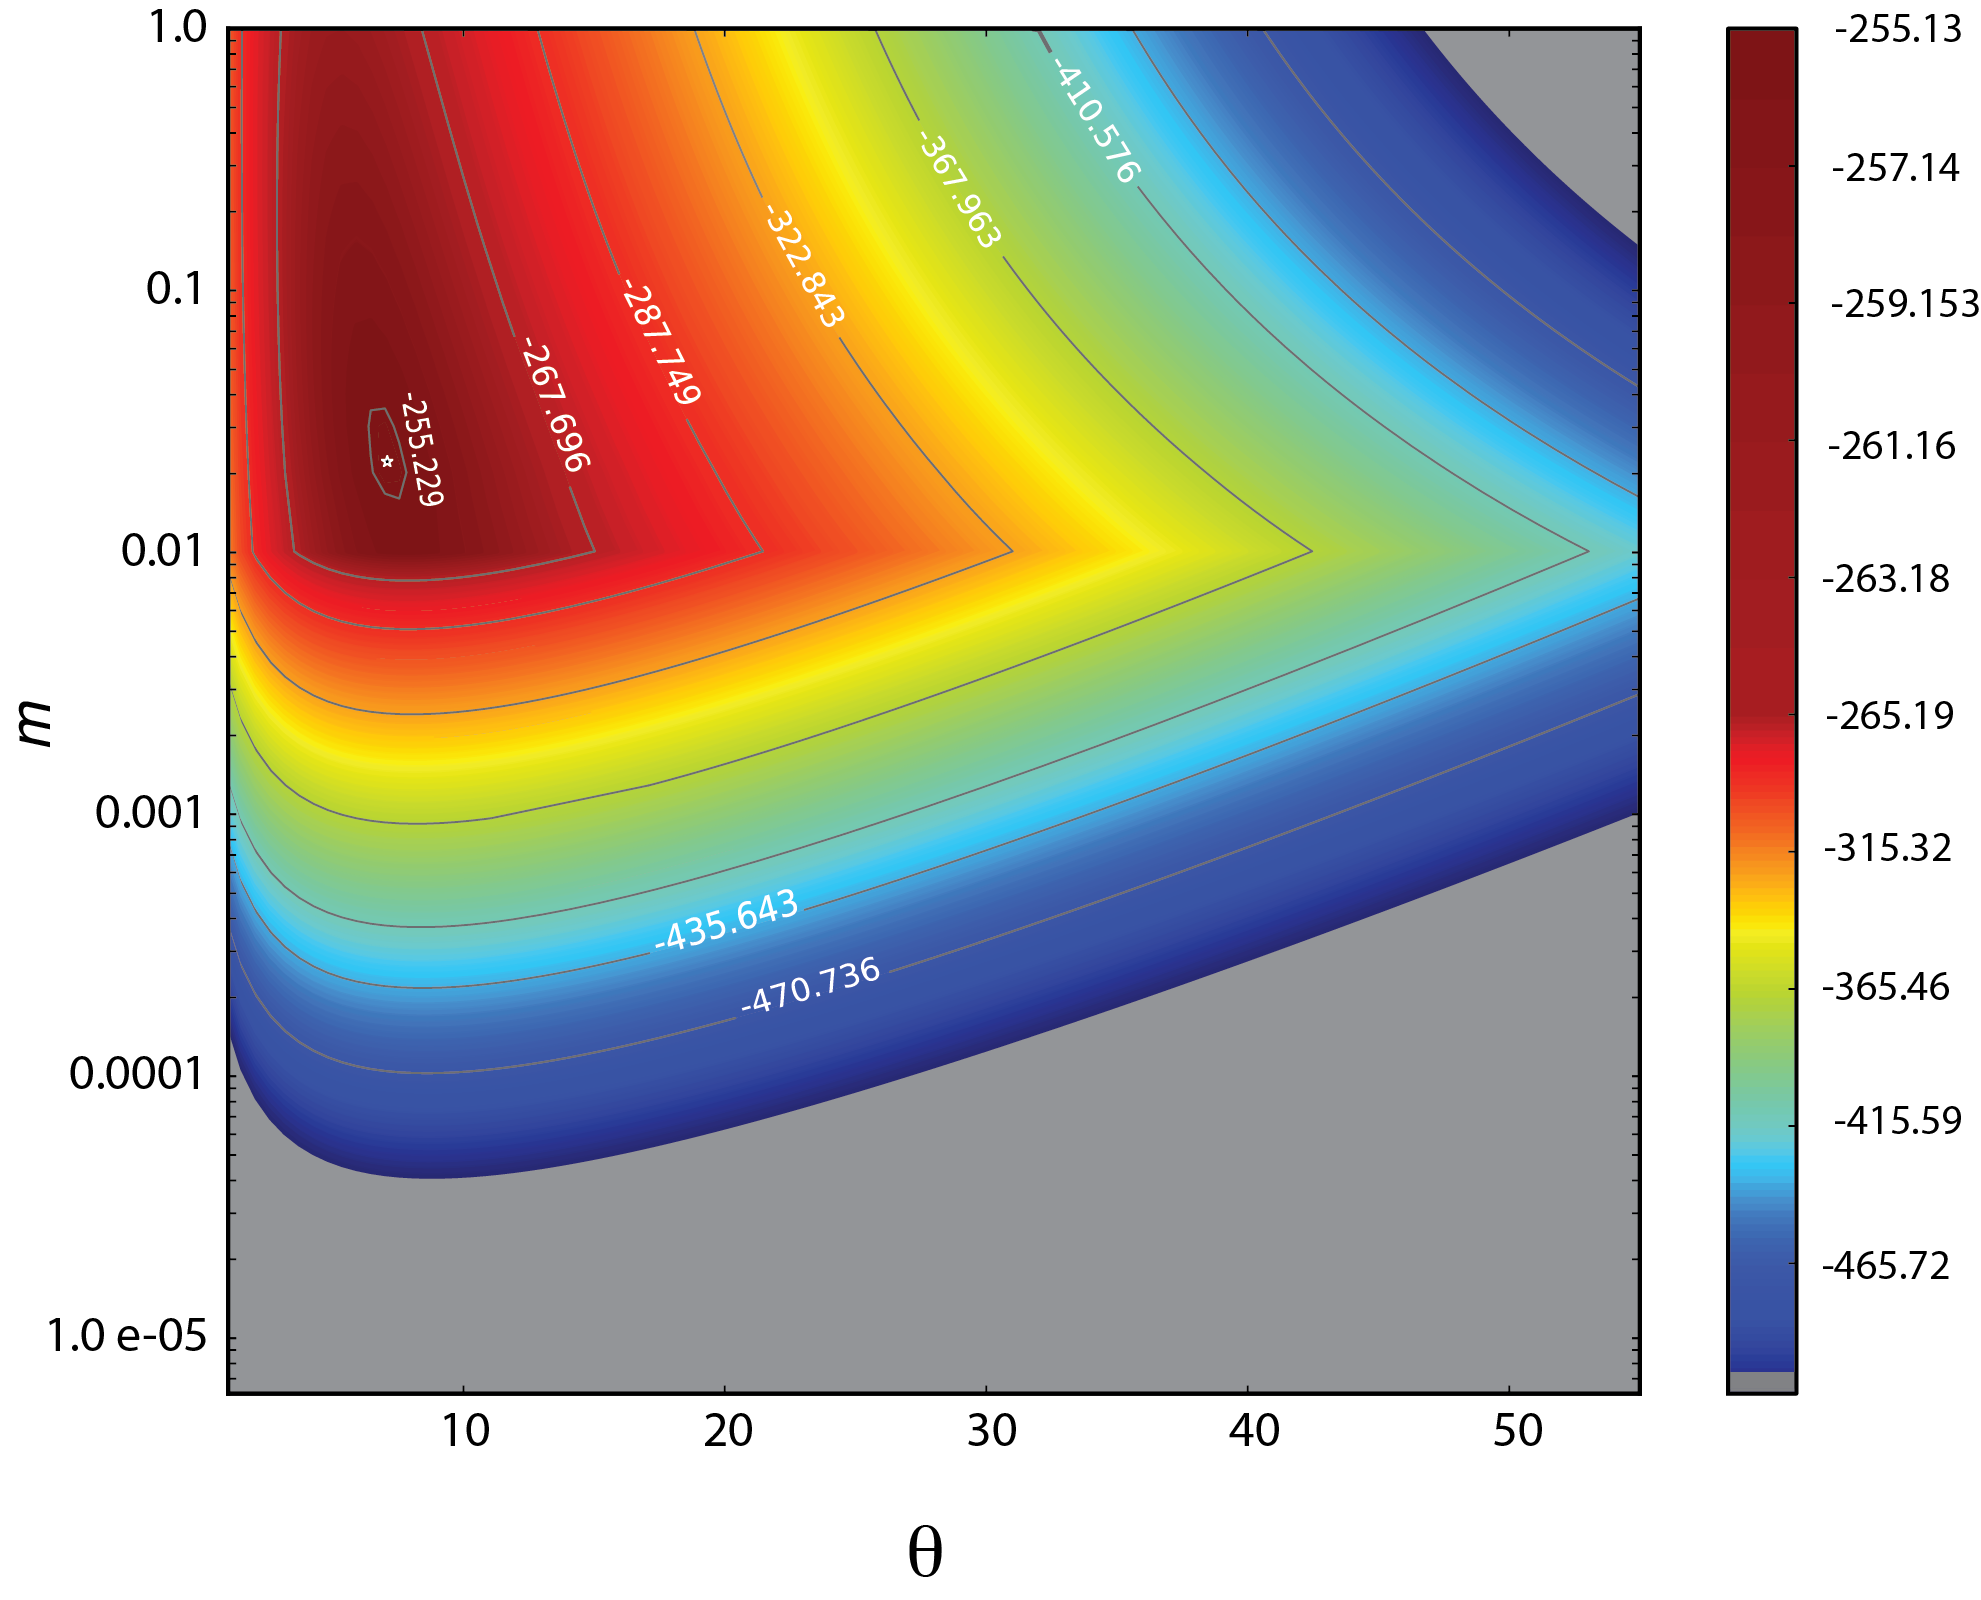
\includegraphics[width=\textwidth]{../figures/untb_genomes/lnl_chrom.png}
\caption[Maximum likelihood inference of neutral parameters.]{{\bf Maximum likelihood inference of neutral parameters.}\\ Log likelihood surface as a function of migration rate ($m$), and the fundamental biodiversity number ($\theta$) for \textit{D. rerio} chromosome 19. Dark red color shows regions of the surface where parameters maximize the probability to explain abundances and diversity of genetic elements in the chromosome. Likelihood ratio tests favored Etienne in contrast to Ewens sampling formula to explain the observed data in the chromosome.}
\label{fig:lnl_chrom}
\end{figure}

\subsection{Model testing}

In order to compare and test the fit of the two models computed, a likelihood ratio test \cite{Wilks1938} was conducted thanks to the fact that Etienne's model is nested into Ewens'. Etienne's model has two free parameters while Ewens' only one (under this model $m$ parameter is fixed to 1), thus the number of degrees of freedom for the chi-squared distribution is 1.

Additionally, given the large number of test performed, statistical significances were corrected by false discovery rate (FDR) \cite{Benjamini2001}. Etienne's model was thus kept as best fit model for only those chromosomes that pass the LRT after FDR adjustment, otherwise the null model using Ewens' formula was selected.

\subsection{Test for neutrality}

In the last years two exact tests were developed in order to accept or reject the neutrality of a given community. Both tests are based on the comparison of a given number of random neutral community generated using the parameters estimated (see \autoref{sec:model-optimization}) for the real data under neutrality. The comparison of the random neutral communities with the observed distribution of abundances, is the key point to test for neutrality.

The first of these tests \cite{Etienne2007} consists in comparing the distribution of likelihoods of fitting neutral model. This corresponding distribution of random neutral abundances is compared to the likelihood of the observed data. The major problem of this test is technical, the computation time needed to optimize the parameters of each abundance distribution and get the likelihoods is unrealistically too high when dealing with GEs.

The second test \cite{Jabot2011} uses, instead of likelihood, the comparison of Shannon's entropy \cite{Shannon1948}, and is much faster as random neutral abundances do not need to be fitted into a neutral model.

Thus, from the neutral parameters obtained for each chromosome, we simulated 10,000 distributions of abundances of GEs and computed, for each,  its Shannon's entropy ($H$). Chromosomes were considered significantly non-neutral when the $H$ of their abundances was below 95\% of the 10,000 random neutral values. As an example \autoref{fig:shannon_distrib}, shows the distribution of H for 10,000 random neutral abundance generated under Etienne's model with $S$, $J$ fixed to the observed numbers and $\theta$ and $m$ corresponding to optimized values for \textit{Anopheles gambiae's} chromosome 2L. In this figure the empirical value of H is below the 95\% of the random neutral distribution, than this chromosome is considered to be non-neutral.

Again, given the high number of tests performed, all p-values obtained from this test were corrected by FDR.

\begin{figure}[htpb]
\centering 
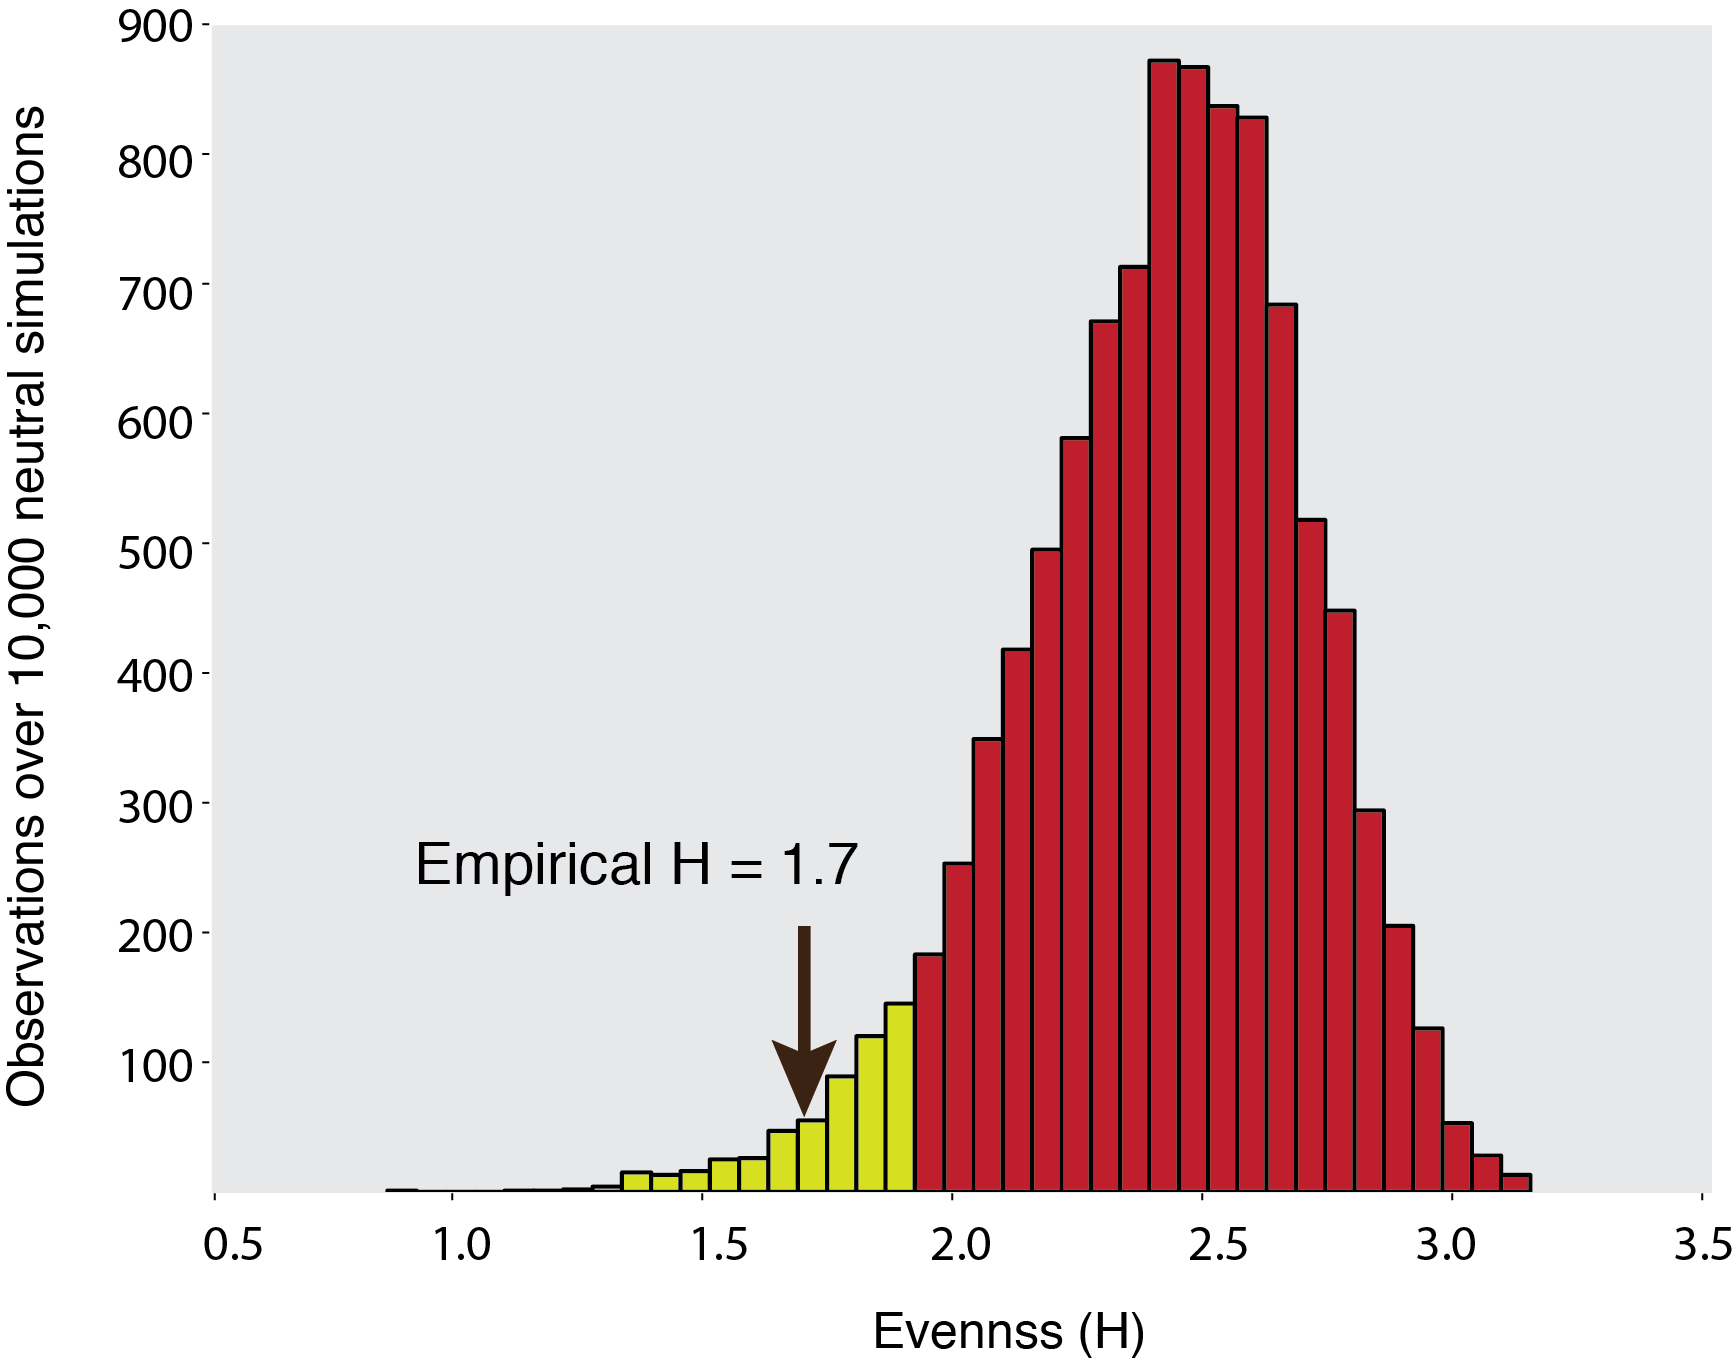
\includegraphics[width=\textwidth]{../figures/untb_genomes/shannon_distrib.png}
\caption[Comparing simulated and empirical evenness.]{{\bf Comparing simulated and empirical evenness. }\\Neutrality test statistically compares simulated null distribution of H with the empirical H value of the corresponding chromosome. In this case, the null distribution of H values was derived from 10,000 neutral simulations of A. gambiae chromosome 2L, with neutral parameters ($\theta$ and $m$) optimized by ML using Etienne sampling formula. Yellow and red bars display 5\% and 95\% of the simulated neutral data, respectively. Although in this case neutrality was rejected (p= 0.01), posterior correction by multiple testing favored the null neutral hypothesis (q= 0.21).}
\label{fig:shannon_distrib}
\end{figure}



\section{Detection of selective pressure at molecular level}
\label{sec:gssa_mat-met}

\subsection{Orthology prediction}

Complete genomes of 5 mammals species (\textit{Homo sapiens}, \textit{Pan troglodytes}, \textit{Mus musculus}, \textit{Rattus norvegicus} and \textit{Canis familiaris}) where retrieved from \textit{Ensembl} \cite{Flicek2011}. Also orthology prediction between each pair of species possibly done between human and the others was retrieved from \textit{Ensembl Compara} \cite{Vilella2009} using biomart \cite{Kinsella2011} and taking human as \mygls{seed} species. Only groups of orthologs \textit{one-to-one} with one representative of each species where kept in the final dataset \fref{fig:phylogeny}{-A}.

\begin{figure}[htpb] 
\centering 
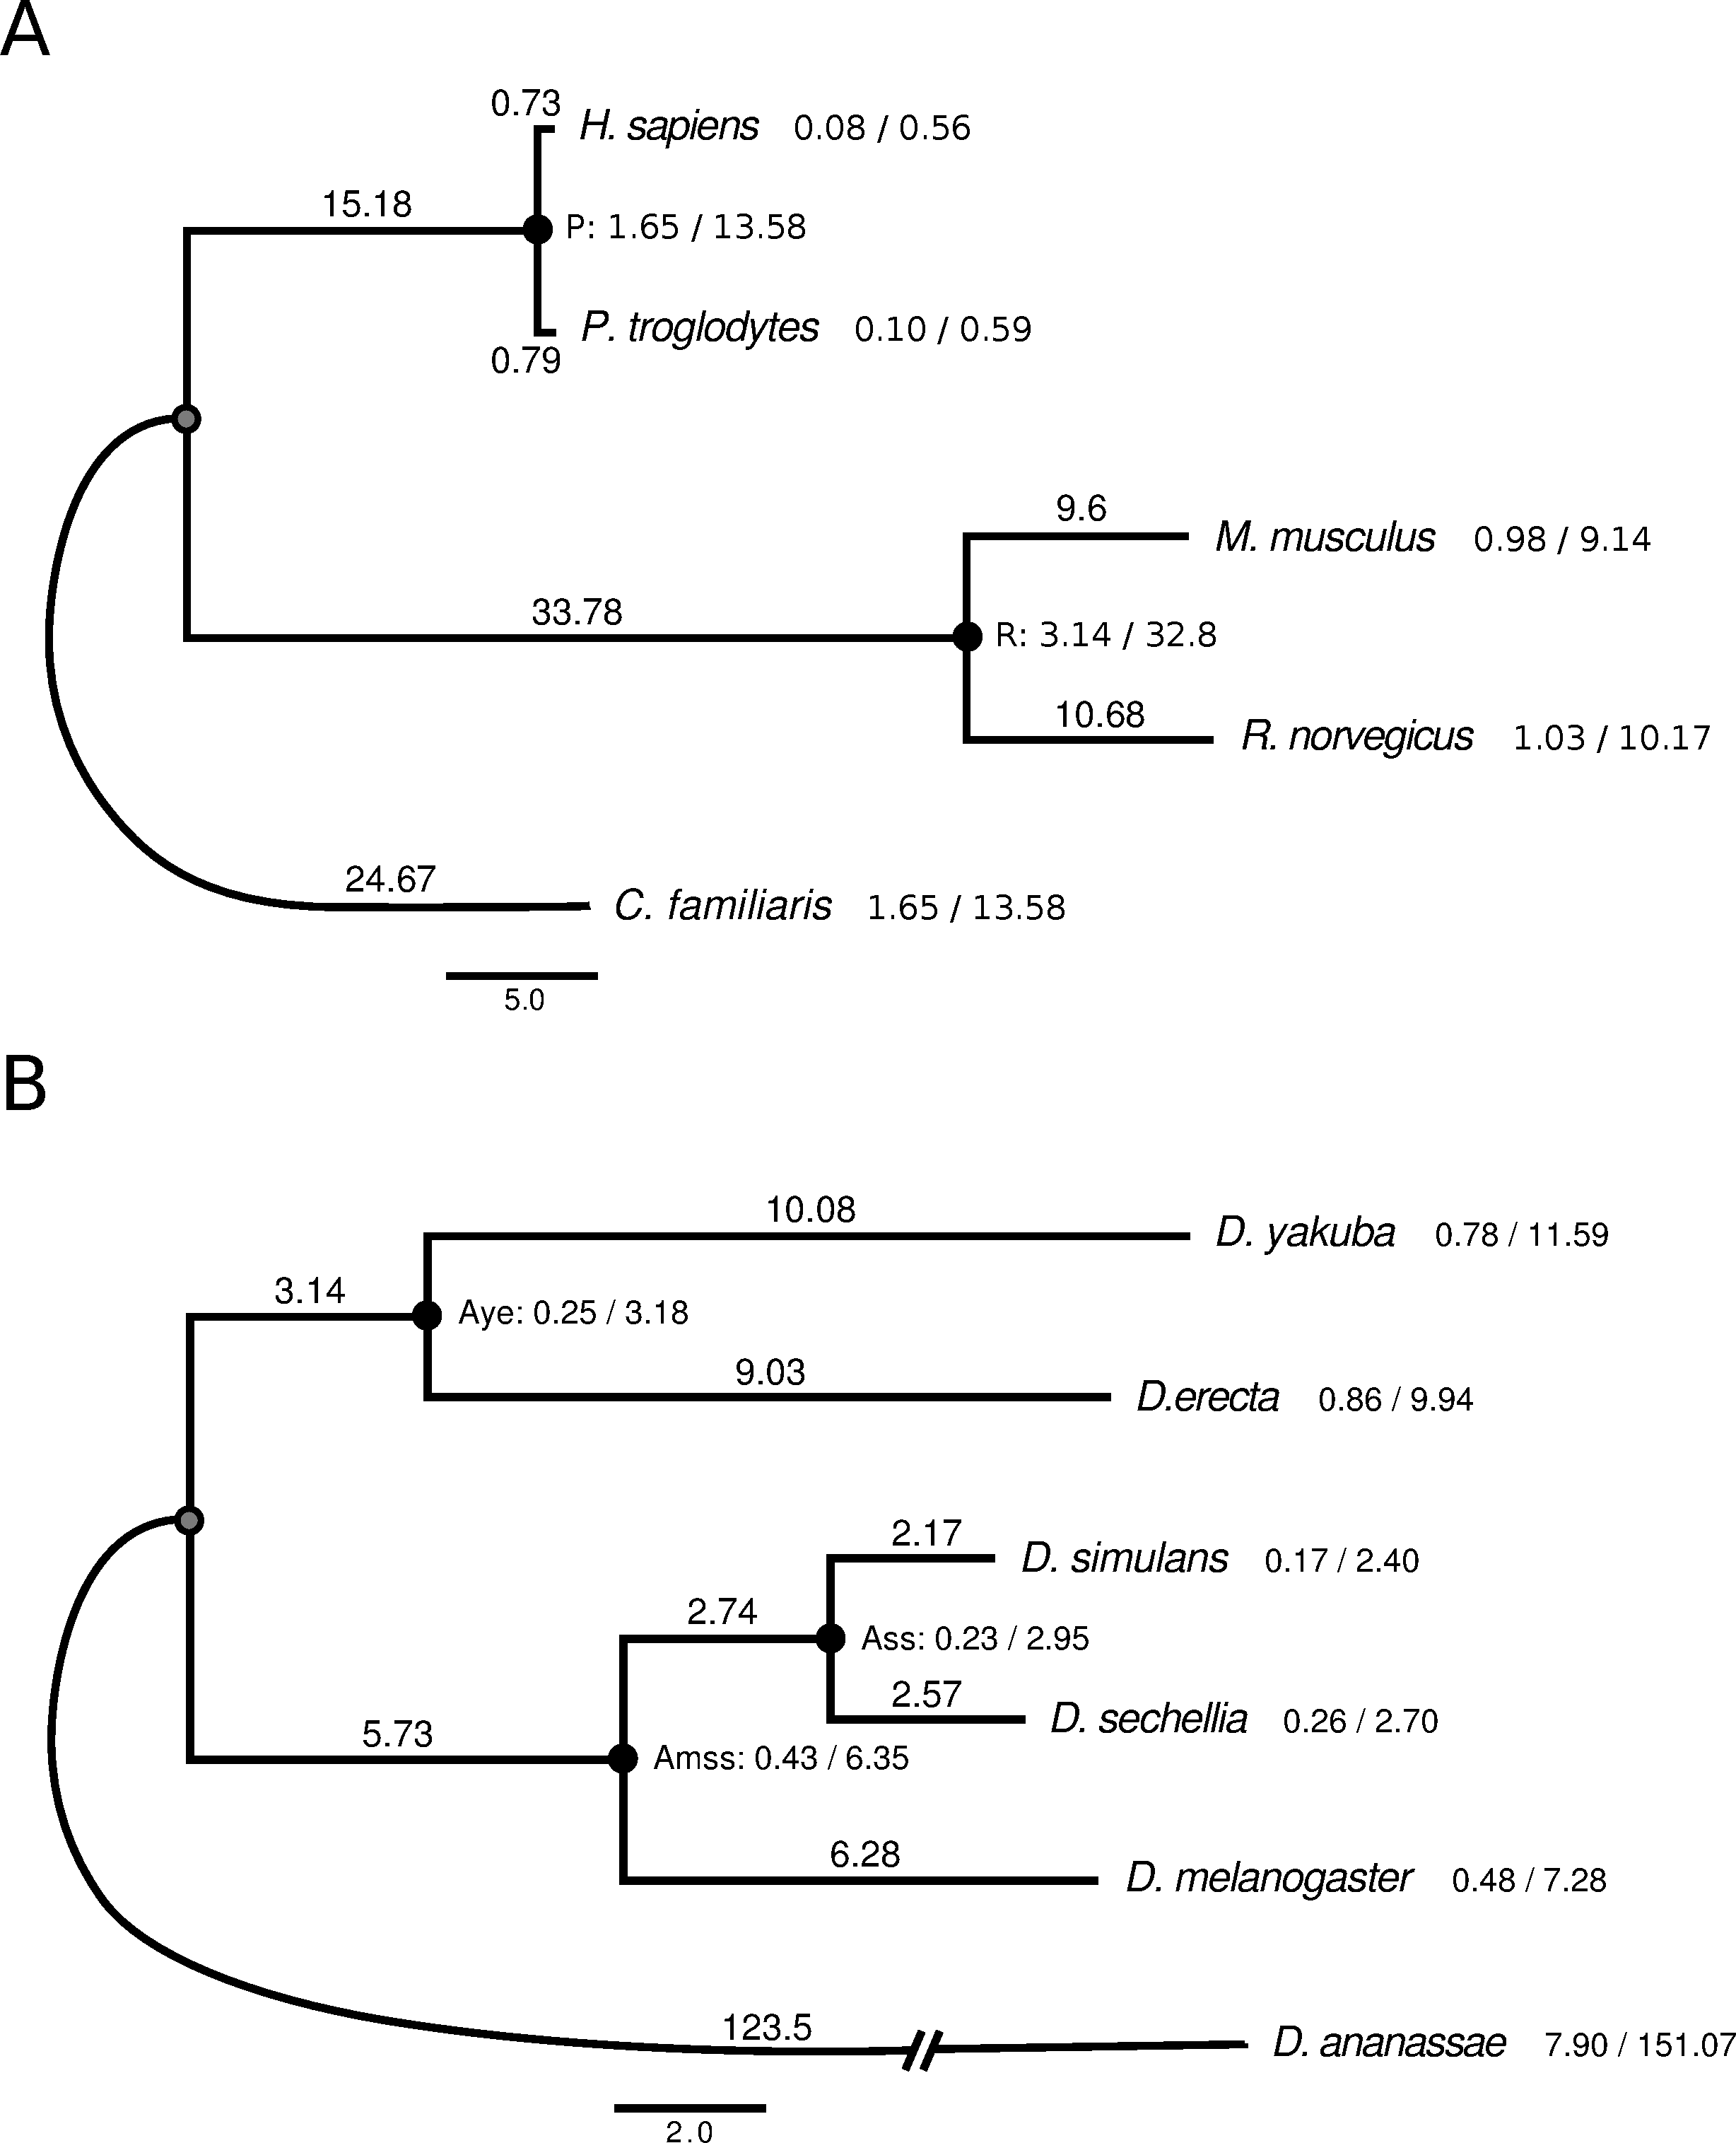
\includegraphics[width=\textwidth]{../figures/gssa/phylogenies.png}
\caption[Mammals and \textit{Drosophila} phylogeny]{{\bf Mammals and
 \textit{melanogaster} group phylogeny.} \\Numbers on internal and external nodes represent the median number of nonsynonymous and synonymous substitutions per codon (dN/dS) estimated from all the coding sequences compared in mammal (A) and Drosophila (B) genomes. Branch lengths and rates were multiplied by 100. Ancestral estimation of parameters was done in primates (P), rodents (R), D. yakuba and D. erecta (Aye), D. simulans and D. sechellia (Ass), and D. melanogaster, D. simulans and D. sechellia (Amss). C. familiaris and D. ananassae were chosen as outgroup species in the corresponding tree.} 
\label{fig:phylogeny}
\end{figure}


The same procedure was applied for \textit{melanogaster} group, including 6 species namely, \textit{Drosophila melanogaster} (as \mygls{seed}-species), \textit{Drosophila sechelia}, \textit{Drosophila simulans}, \textit{Drosophila yakuba}, \textit{Drosophila erecta} and, as outgroup, \textit{Drosophila ananassae} (see \fref{fig:phylogeny}{-B}).

\subsection{Alignments refinement and filters}
DNA coding sequences (CDS) were aligned according to protein translation pattern using \textit{Muscle} version 3.7 \cite{Edgar2004} embedded into the \textit{CDS-Protal} utility in \textit{Phylemon 2.0} \cite{Sanchez2011}, and to avoid the presence of badly aligned regions alignments were cleaned using \textit{TrimAl} \cite{Capella-Gutierrez2009} keeping all sequences but trimming alignment columns with the heuristic method \textit{automated-1}. Additionally, alignments smaller than 100 bp were excluded from the analysis. 

In mammals, the upper limit for dN and dS considered was those of the human interferon $\gamma$ (dN = 3.06) and the relaxin protein \cite{Graur2000} (dS = 6.39 substitutions per site per 1e9 years). Assuming the human-mouse, mouse-rat and human-chimp differentiation times to be about 80, 70 and 5 million years \cite{BlairHedges2003}, respectively, ortholog comparisons between primates and rodents with dS$\ge$1 and dN$\ge$0.5, rodents with dS$\ge$0.256, dN$\ge$0.122, and primates with dS$\ge$0.064 and dN$\ge$0.030 substitutions/site were excluded.

The number of orthologs kept for analysis after filtering steps, is 12,453 for mammals, and 9,240 for flies.

\subsection{Evolutionary analysis}

Maximum likelihood estimation of dN, dS, and $\omega$ was computed using CodeML program from PAML \cite{Yang2007}. Evolutionary rates were computed in orthologous sequences according to the free-ratio branch model assuming independent $\omega$ ratio for each branch of the tree of mammals and Drosophila species (see raw values of rates in Table S1 and S2). Evolutionary rates (dN, dS), its ratio ($\omega$), and its difference between ancestral and descendant species ($\Delta\omega$) were ranked along all genes of genomes and further analyzed by GSSA.

External branches of Figure 1 were labeled as foreground to test for positive selection using branch-site models in Test I and Test II \cite{Zhang2005}. Positive results of relaxation of selective constraints (or weak signals of positive selection) were discarded \cite{Arbiza2006}. To quantify the relative contribution of PSGs in functional modules showing SH$\omega$ and SL$\omega$ results in GSSA, a t-test (from R package \cite{Ihaka1996}) with the mean number of PSGs per functional modules was computed in primates, rodents, mammals and Drosophila species. An independent set of PSGs was collected to test the robustness of our results in mammals \cite{Kosiol2008a}, and Drosophila species \cite{Clark2007}.

\subsection{GSSA, evolutionary and statistical simulations}

Gene-set selection analysis across lists of genes ranked by different evolutionary rate parameters (dS, dN, $\omega$ and $\Delta\omega$) was computed using the program Babelomics \cite{Al-Shahrour2008}. This program implements a version of GSA \cite{Al-Shahrour2005a} which can be applied to any list of ranked genes regardless of the initial experimental design \cite{Dopazo,Huang2009}. The aim of the test is to find functional classes, namely blocks of genes that share some functional property, showing a significant asymmetric distribution towards the extremes of a list of ranked genes. This is achieved by means of a segmentation test, which consists on the sequential application of a Fisher's exact test over the contingency tables formed with the two sides of different partitions (A and B in \autoref{fig:gssa_met}) made on an ordered list of genes. The two-tailed Fisher's exact test finds significantly over or under represented functional classes when comparing the upper side to the lower side of the list, as defined by any partition (in \autoref{fig:gssa_met}, four of the five partitions show significant differences). Similarly to other equivalent gene-set analyses, the outcomes are those modules (GO and KEGG) significantly associated to high or low values of the evolutionary parameter used to rank the genes. Previous results showed that a number between 20 and 50 partitions often gives optimal results in terms of sensitivity and results recovered \cite{Al-Shahrour2005a}. Here we applied 30 partitions along all the GSSA performed. Given that multiple functional classes (C) are tested in multiple partitions (P), the unadjusted p-values for a total of C $\cdot$ P tests were corrected by the widely accepted FDR method \cite{Benjamini2001}.

\begin{FPfigure}
\centering 
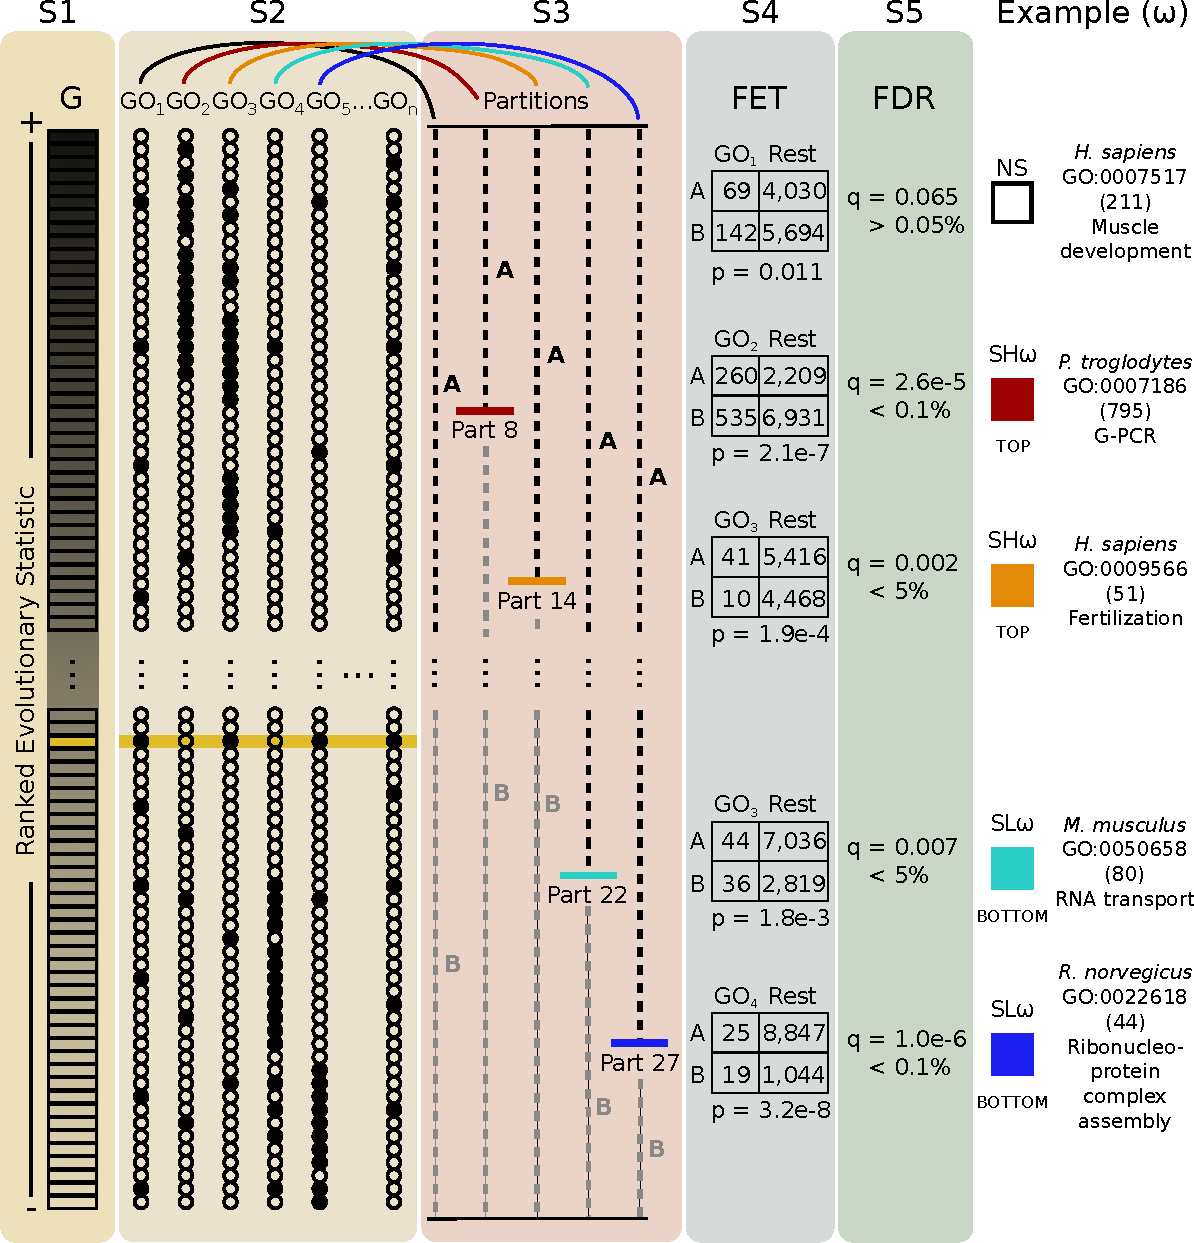
\includegraphics[width=\textwidth]{../figures/gssa/gssa_met.pdf}
\caption[Summary of the steps developed by the GSSA.]{{\bf Summary of the steps developed by the GSSA.} \\GSSA can be roughly described in a series of five steps (S1 to S5). S1: rank genes of a genome according to an evolutionary variable, S2: assign functional classes to all the listed genes, S3: apply a fixed number of partitions on the ranked list, S4: proceeds with a Fisher exact test (FET) for each partition, S5: adjust p-values by FDR. See text for a full description. Colored boxes (red, orange, cyan and blue) represent functional modules with genes significantly accumulated (0.1\% FDR and 5\% FDR) at the corresponding extremes of a list (top and bottom), and therefore with significantly high (SH) and low (SL) values of the evolutionary variable ($\omega$) respectively. White represents a non-significant association (NS). Examples show five alternative GO categories with significant and non-significant distributions of the $\omega$ statistic. In parenthesis, the total number of genes corresponding to the GO term is shown. For GO1, the function seems to be uncorrelated with the arrangements of the genes. In the example (GO:0007517) partition 16 in human (not shown in the picture) reported the lowest p-value (p = 0.011) although it was not significant after FDR correction (FDR = 0.065). Upper (A) and lower (B) sides of the ranked list (S3) represent both sides of the specified partition number. Remainder GO categories (GO2 to GO5) show the association of dark dots with values located at the top (significant high $\omega$ values -SH$\omega$), and at the bottom (significant low $\omega$ values -SL$\omega$) of the list (for GO2-GO3 and GO4-GO5, respectively). In examples, FETs found the most significant p-value for partitions 8, 14, 22 and 27 for GO:0007517, GO:0007186, GO:0009566, GO:0050658 and GO:0022618 in chimpanzee, human, mouse and rat genome, respectively.}
\label{fig:gssa_met}
\end{FPfigure}

Originally, 1,394/1,331 GO terms, and 199/116 KEGG pathways were analyzed in mammals and Drosophila species respectively. The global GO directed acyclic graph was processed with Blast2GO \cite{Conesa2005} to extend the annotation at missing parental nodes, discarding GO levels out of 2 to 8 for mammals, and 2 to 12 for Drosophilas. The final set of GO and KEGG terms used in the GSSA corresponds to those containing a minimum number of 15 genes. To test possible biases attributed to the size of the functional category, the magnitude of change in evolutionary rate or the proportion of genes experiencing a rate change we randomized the original assignation of ENSG's to the list of ranked values and functional annotation (see \fref{fig:gssa_simul}{-A}). For each evolutionary variable and species 10.000 randomizations and the corresponding GSSA were performed. The proportion of false positives (significant results after GSSA) was computed for each evolutionary variable and plotted along the size of functional categories (from 20 to 1,400 with intervals of 20). Because this proportion never reached values higher than 0.5\% (FDR) we rejected the possibility that either group size or rate distribution biased GSSA results in our data set (see \fref{fig:gssa_simul}{-B} and \fref{fig:gssa_simul}{-C}).

\begin{FPfigure}
\centering 
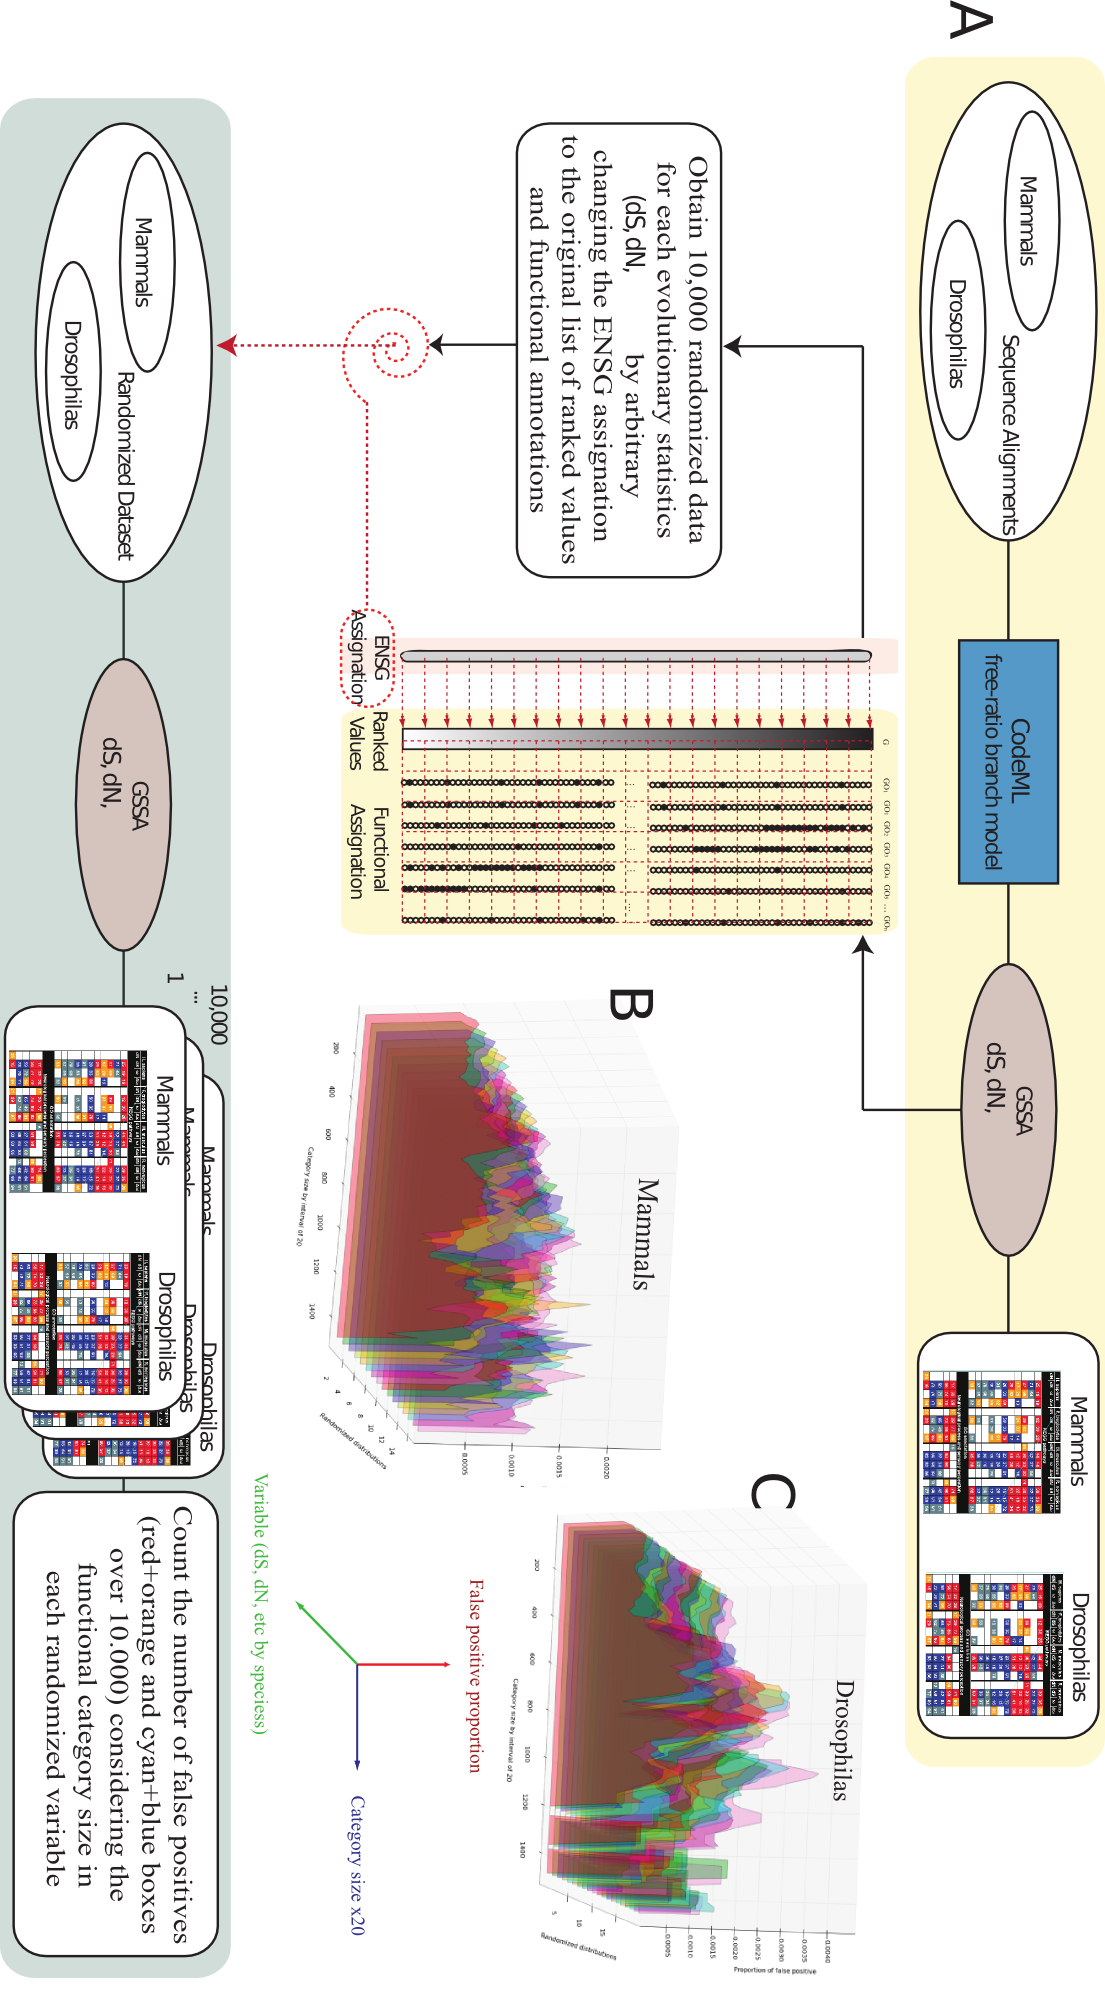
\includegraphics[height=\textheight]{../figures/gssa/gssa_simulations.png}
\caption[Randomisation experiment.]{{\bf Randomisation experiment.} \\(A) The pipeline shows the steps followed to tests possible biases attributed to the size of the functional category, the magnitude of change in evolutionary rate and the proportion of genes experiencing a rate change in the GSSA. The proportion of false positive results never reached 5\% (FDR) in mammals (B) and Drosophila (C).}
\label{fig:gssa_simul}
\end{FPfigure}

Finally, in order to validate the independence of the GSSA from the effects of alternative evolutionary constraints we simulated selective regimes (purifying selection, positive selection and relaxation of selective constraints) using branch-site models. Here we addressed the possibility of a variation in the representation of significant results after GSSA (see \autoref{fig:gssa_simul_pipe}). The pipeline described here, shows three different areas: 
\begin{itemize}
\item \textbf{Real Data}: the dark yellow area describes the steps used to reach to results described in the manuscript. The light yellow area describes the use of the CodeML program from PAML package (reference 15 in the ms) to extract -from the original set of sequences -the evolutionary parameters to simulate new sequences under purifying selection (PF), positive selection (PS) and relaxation of the selective constraints (RX) using branch-site models (see model description below). Human, mouse, \textit{D. erecta} and \textit{D. melanogaster} were used as foreground species in the corresponding models.
\item \textbf{Simulated Data}: Evolver (PAML program) simulates sequences using parameters (codon frequencies and branch lengths) from the empirical data. We checked the desired characteristics of positive selection (PS) and relaxation of selective constraints (RX) on the set of the simulated sequences \autoref{tab:psg_simul}. Evolutionary variables (dS, dN, $\omega$ and $\Delta\omega$) were estimated from simulated sequences by means of a free-ratio branch model (CodeML). The complete pipeline of the GSSA was applied in the simulated data.
\item \textbf{Testing simulation}: The odd-ratio of the values observed on the contingency table of each significant functional term after GSSA was computed. Values higher and lower than one contribute to the total number of functional modules with significant high and low $\omega$ values. To test the statistical contribution of these functional modules to these extremes on the simulated regimes (PS, RX and PF) the log odd-ratios were compared using t-test.
\end{itemize}

\begin{figure}
\centering 
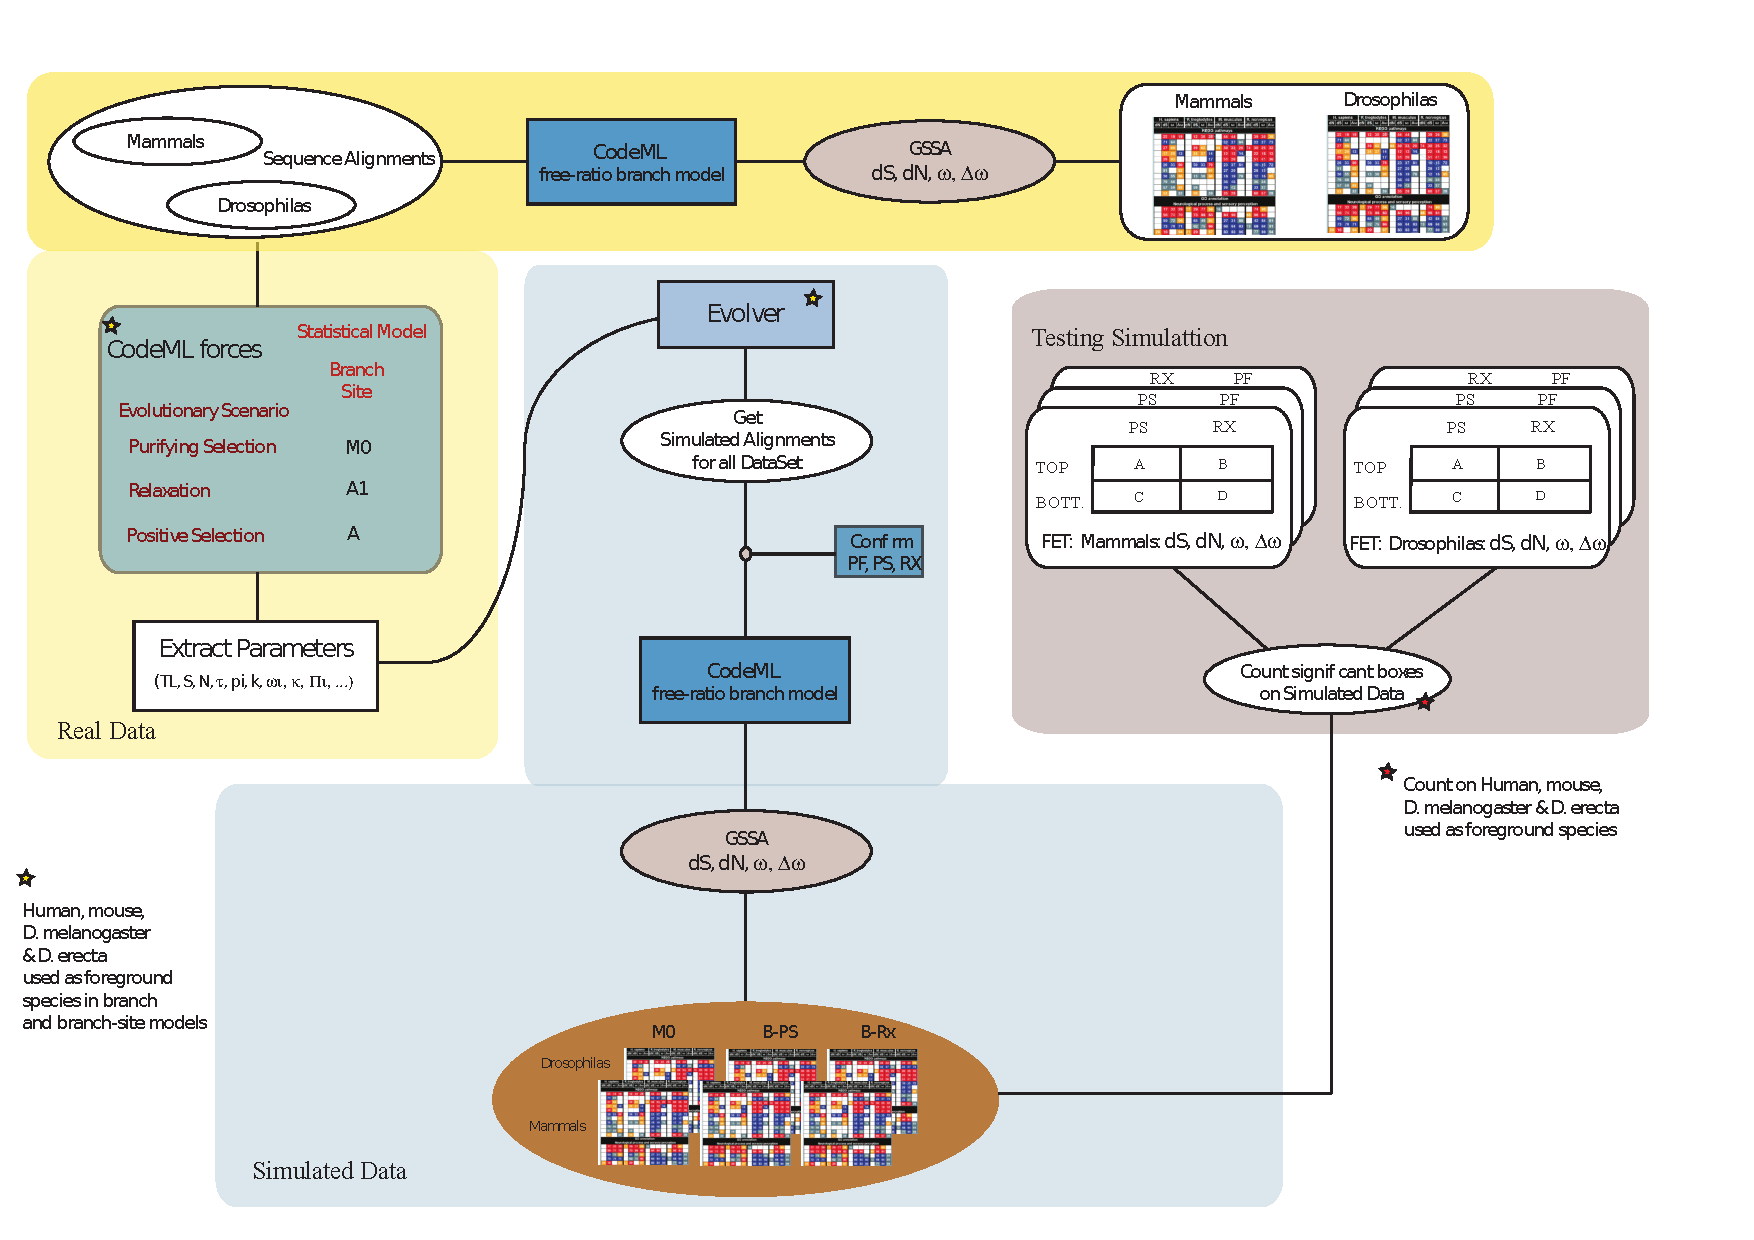
\includegraphics[width=\textwidth]{../figures/gssa/gssa_simulations_pipeline.pdf}
\caption[Evolutionary and statistical simulation of GSSA.]{{\bf Evolutionary and statistical simulation of GSSA.} \\ The pipeline shows the steps taken along three different spaces of analysis, the real data, the simulated data and the testing block. See Supplementary Results for a complete explanation of methods and results.}
\label{fig:gssa_simul_pipe}
\end{figure}

\rowcolors{1}{white}{white}
\begin{table}[htbp]
\resizebox{\textwidth}{!}{%
\begin{tabular}{l r r r r r r}
\multicolumn{1}{l}{} & \multicolumn{ 2}{c}{PS} & \multicolumn{ 2}{c}{RX} & \multicolumn{ 2}{c}{PF} \\ \hline
\multicolumn{1}{l}{} & \multicolumn{1}{c}{\# PSG} & \multicolumn{1}{c}{\# RXG} & \multicolumn{1}{c}{\# PSG} & \multicolumn{1}{c}{\# RXG} & \multicolumn{1}{c}{\# PSG} & \multicolumn{1}{c}{\# RXG} \\ \hline
Homo sapiens & 658 & 1640 & 11 & 1939 & 0 & 1 \\
Mus musculus & 1500 & 954 & 14 & 1565 & 1 & 0 \\
D. melanogaster & 736 & 630 & 25 & 1104 & 0 & 0 \\
D. erecta & 778 & 1292 & 26 & 1713 & 2 & 1 \\ \hline
\end{tabular}
}
\caption[Number of PSG and relaxed genes (RXG) in each of the simulated evolutionary scenarios]{Number of PSG and relaxed genes (RXG) in each of the simulated evolutionary scenarios.}
\label{tab:psg_simul}
\end{table}

Our results showed that in spite of the alternative evolutionary scenarios no significant differences were observed between log odd-ratios distribution (p<0.05). This result is exactly what we expected. The average effect of PF, and RX-PS is the proportional decrease and increase of the mean value of $\omega$ on sequences, respectively. This change has minor effects (if any) in the relative position of genes in the ranked list of genes of a genome. Accordingly, since no net differences were produced after ranking genes, no significant differences are expected after the t-test (PS-RX: p= 0.99, PS-PF: p= 0.45, and RX-PF: p= 0.46). The fact that basically the same number of significant results was observed in each evolutionary scenario confirmed this prediction \autoref{tab:prop_signif}. We conclude that neither of the selective regimes simulated produce significant differences or biases in the GSSA of $\omega$ values.


\begin{table}[htbp]
\begin{center}
\begin{tabular}{l c c c}
\hline
 & PS & RX & PF \\ \hline
PS & --- & 92.50\% & 98.50\% \\
RX & 91.10\% & --- & 99.00\% \\
PF & 88.90\% & 90.60\% & --- \\ \hline
\end{tabular}
\end{center}
\caption[Proportion of significant functional categories that are still significant.]{Proportion of significant functional categories that are still significant (identical signs of odd-ratios) under a different evolutionary scenario.}
\label{tab:prop_signif}
\end{table}





%%% Local Variables: 
%%% mode: latex
%%% TeX-master: "../thesis_main"
%%% End: 

\message{ !name(../thesis_main.tex) !offset(-487) }

\end{document}

%%% Local Variables:
%%% mode: latex
%%% TeX-master: t
%%% End: 
